%% Tudor
\begin{frame}
  \frametitle{What is Machine Learning?}
  \begin{block}{Machine Learning}
    A computer program is said to learn from experience $E$ with
    respect to some class of tasks $T$ and performance measure $P$, if
    its performance at tasks in $T$, as measured by $P$, improves with
    experience $E$.
  \end{block}
\end{frame}

\begin{frame}
  \frametitle{Machine Learning Applications}
  \begin{itemize}
  \item Computer Vision: Google Car
  \item Machine Translation
  \item Speech Recognition
  \item Recommender Systems
  \item Intelligent Advertising
  \end{itemize}
\end{frame}

\begin{frame}
  \frametitle{Machine Learning Classification}
  Types of Machine Learning Problems
  \begin{columns}
    \column{0.7\textwidth}
    \begin{itemize}
    \item Regression
    \item Classification
    \item Reinforcement Learning
    \end{itemize}
    \begin{itemize}
    \item supervised learning (eg. ..)
    \item unsupervised
    \end{itemize}
    \column{0.3\textwidth}
    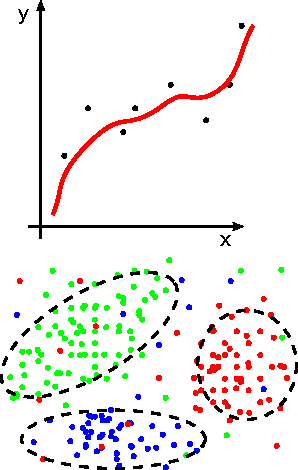
\includegraphics[width=\textwidth]{graphics/ml-intro/ml.pdf}
  \end{columns}
\end{frame}
